\documentclass[12pt,a4paper]{article}

% --- Настройка языка и шрифтов (для XeLaTeX) ---
\usepackage{fontspec}
\setmainfont{Times New Roman} % Основной шрифт (можно заменить на Computer Modern)
\usepackage{polyglossia}
\setdefaultlanguage{russian}
\setotherlanguage{english}
\usepackage{cancel}
\usepackage[normalem]{ulem}

\hyphenpenalty=10000
\exhyphenpenalty=10000
\sloppy

% --- Поля и геометрия страницы ---
\usepackage[left=25mm,right=20mm,top=20mm,bottom=20mm]{geometry}

% --- Математические пакеты ---
\usepackage{amsmath,amssymb,amsthm,mathtools}
\usepackage{bm} % Жирные математические символы через \bm{}

% --- Настройка теорем и определений ---
\theoremstyle{plain} % Стиль для теорем, лемм (курсив)
\newtheorem{theorem}{Теорема}[section]
\newtheorem{lemma}[theorem]{Лемма}
\newtheorem{proposition}{Предложение}
\newtheorem{corollary}{Следствие}

\theoremstyle{definition} % Стиль для определений и примеров (прямой шрифт)
\newtheorem{definition}{Определение}[section]
\newtheorem{example}{Пример}[section]

\theoremstyle{remark} % Стиль для замечаний
\newtheorem{remark}{Замечание}

% Кастомный символ окончания доказательства
\renewcommand{\qedsymbol}{$\blacksquare$}

% --- Ссылки и гипертекст ---
\usepackage[colorlinks=true, linkcolor=blue, citecolor=blue, urlcolor=blue]{hyperref}

\begin{document}
	\section{Двумерные динамические раскраски}
	\begin{definition}
		Динамическая r-раскраска - это правильная раскраска графа, где у каждой вершины степени не менее r имеется хотя бы r соседей с попарно различными цветами.\\
		
		$\chi_r(G)$ - Минимальное число цветов, для которых существует r-динамическая раскраска. Отметим, что в таких обозначениях можно считать $\chi(G) = \chi_1(G)$
		
		Стандартные обозначения: $G = (V, E)$ - граф; $v_i, a_i$ - вершины; $\Delta, \Delta(G)$ - максимальная степень вершины; $N_G(v)$ - окрестность вершины, т.е. все вершины смежные данной; $v(G)$ - число вершин в графе; $M = \{1, ..., n\}$ - множество цветов; $\rho:V\rightarrow M$ - раскраска вершин
		
	\end{definition}
	
	\begin{lemma}.
		\\$\boxdot \chi_2(G) \leq \Delta(G) + 1, \space \Delta(G) \geq 4$\\
		$\boxdot$ Вероятно, результат можно обобщить: $\chi_r(G) \leq \Delta(G) + r - 1, \space r \leq \Delta(G), \space \Delta(G) \geq 4$\\
		$\boxdot$ Оценку можно улучшить: $ \chi_2(G) \leq \Delta(G), \space \Delta(G) \geq 5$. Если граф не является полным.\\
		$\boxdot$ Вероятно, можно обобщить: $\chi_r(G) \leq \Delta(G) + r - 2, \space r \leq \Delta(G), \space \Delta(G) \geq 5$\\
	\end{lemma}
	$\triangleright$
	\boxed{\chi_2(G) \leq \Delta(G) + 1, \space \Delta(G) \geq 5}
	\begin{itemize}
	\item Индукция по $v(G)$.
	\item База: несвязный или пустой граф. Для него подойдет раскраска в один цвет, правильность и динамичность которой проверять не нужно.
	\item Переход: $v(G)\mapsto v(G)+1$
	\item Индукция будет действовать так: будем удалять вершину графа и по индукционному предположению раскрашивать динамически подграф, а далее возвращать удалённую вершину и проверять правильность и 2-динамичность только для этой вершины. Если правильно перестроить подграф, то оба свойства будут получаться автоматически.
	\item Везде считаем - что удаляем вершину $v$, $N_G(v) = \{a_1, ..., a_n\}$ и $H = G-v$
	\item Сначала разберём тривиальные случаи:
	\item Пусть существует вершина $v$ степени 1, тогда удалим её и по индукционному предположению раскрасим подграф. 
	\item Единственный сосед $a_1$ удаленной вершины $v$ в графе $H$ либо имеет двух соседей, тогда 2-динамичность $a_1$ гарантирована индукцией. Иначе - всегда получится выбрать цвет для вершины $v$, чтобы получить правильность и 2-динамичность.
	\item В случае если есть вершина $v$ степени 2: $N_G(v) = \{a_1, a_2\}$, тогда достаточно заменить её на ребро $a_1a_2$ (если его нет в G) и удалить из графа саму $v$. Тогда это ребро гарантирует 2-динамичность.
	\item Осталось понять, в какой цвет покрасить вершину $v$ в случае, если вершины $a_1, a_2$ имели степень 1 в графе $H$. Для этого введём интуитивное понятие:\\
	$\blacksquare$  Вершина "запрещает" цвет $k$, если при покраске её не раскрашенного соседа в этот цвет раскраска потеряет правильность или 2-динамичность.\\
	\item Отметим важное свойство: каждая вершина может запрещать не более двух цветов (один по правильности и ещё один по динамичности)
	\item Так вот, имеется два соседа, каждый запрещает два цвета. Следовательно в общем случае нам потребуется хотя бы 5 цветов, чтобы не было конфликтов с вершинами $a_i$. 
	\item Кажется больше нигде не будет требоваться условие, на наличие хотя бы 5 цветов в раскраске.
	\item 2-Динамичность самой вершины $v$ тривиально следует из наличия ребра $a_1a_2$ в графе H и правильности раскраски $\rho_H$.
	\item Первые два разобранных случая можно считать приоритетными при выборе шага индукции. Опишем теперь случай $\delta(G) \geq 3$. Далее будет удобно ввести ещё одно понятие:\\
	$\blacksquare$ "Вырезание" вершины $v$ из графа: удалим вершину $v$ из графа. Далее разобъем всю окрестность на пары, возможно одна вершина не войдёт ни в одну пару (но хотя бы одна пара точно будет, благодаря условию $\delta(G) \geq 3$). В каждой (или хотя бы одной, сейчас это не важно) паре $a_i, a_j$ проведём ребро $a_ia_j$ взамен удалённой вершины.\\
	Отметим, что при такой операции максимальная степень $\Delta$ не возрастёт.
	\item Если в графе есть треугольник $va_1a_2$ - удалим вершину $v$ этого треугольника, далее по индукции динамично перекрасим полученный подграф и вернём вершину. 2-Динамичность самой $v$ гарантируется уцелевшем в подграфе H ребром $a_1a_2$. Правильность раскраски $v$ следует из наличия одного запосного цвета - раскрасить правильно мы сможем всегда.
	\item Осталось проверить 2-динамичность вершин $a_1, a_2, a_3, ..., a_n$
	\item После удаления вершины $v$ степень каждой из вершин $a_i$ упала ровно на 1. То есть $\delta_H(a_i) = \delta_G(a_i) - 1 \geq 2$, т.е. все $a_i$ 2-динамичны ещё в графе H.
	\item Последний вариант, в графе нет треугольников. Тогда создадим его сами: "вырежем" вершину $v$ добавив хотя бы одно ребро, НУО $a_1a_2$ - оно гарантирует 2-динамичность.
	\item Доказательство корректности последнего построения полностью аналогично пункту про наличие треугольника в графе.
	\end{itemize}
	\hfill $\square$\\
	\boxed{\chi_r(G) \Delta(G) + r - 1, \space r \leq \Delta(G)-1, \space \Delta(G) \geq 4,r}
	$\triangleright$
	\begin{itemize}
		\item Доказательство аналогичное, случаи $d_G(v) \in \{1, 2\}$ - полностью аналогичные, поэтому достаточно рассматривать случай $\delta \geq 3$
		\item Далее, если в графе не осталось вершин степени $d_G(v) \geq r$ - то это базовый случай и доказательство окончено
		\item Значит такая вершина есть: случаи наличия треугольника и его отсутствия модифицируются так:
		\item Если вершина $v$ смежна клике хотя-бы на $r$ вершинах, то r-динамичность самой $v$ очевидна. 
		\item r-Динамичность вершин $a_i$ степени хотя-бы $r+1$ тоже очевидна, т.к. в графе $H = G-v$ они будут иметь степень $r$ и будут r-динамично раскрашены по предположению
		\item Значит нас волнуют только вершины $a_i$ степени ровно $r$. Каждый такой сосед запрещает\\
		---------------------------------нз----------------------
		видимо надо двигать границу на $\Delta$
	\end{itemize}
	\hfill $\square$\\
	\boxed{\chi_2(G) \leq \Delta(G), \space \Delta(G) \geq 5}
	\begin {itemize}
	\item Доказательство снова повторяет процесс индукции из первого пункта.
	\item Поэтому сразу считаем, что $\delta(G) \geq 3$
	\item Воспользуемся леммой о галке. Для этого нужно прийти к двусвязности графа.
	\item Переход индукции в случае несвязности графа очевиден
	\item Если в G есть точка сочленения - удаляем её. Склеить правильно и 2-динамично раскраски получившихся компонент связности очевидно можно.
	\item Если существует вершина степени, меньшей, чем максимальная: $d_G(v) < \Delta(G)$ то её можно раскрасить по индукции из первого пункта, не выходя за границу $\chi_2(G) \leq \Delta(G)$, так что достаточно рассмотреть случай, когда граф G - регулярный, но не полный.
	\item Т.о.: рассматриваем случай G - двусвязный и применяем лемму, т.е. $H = G-a-c$ - связен, $va,vc \in E, ac \cancel{\in} E$
	
	\item Далее рассмотрим два случая:
	\item Случай 1: $(N_G(a) \cap N_G(c))\setminus v \cancel= \emptyset$ - пусть это вершина $u$
	\item Тогда удалим весь квадрат $a, v, c, u$. Если существует вершина, смежная со всем квадратом, то её степень упадёт на 4. А значит, чтобы не бояться за её 2-динамичность нам потребуется ограничение $\Delta(G) \geq 6$. Это ограничение можно улучшить: если она смежна с этим квадратом, то правильно раскрашенный квадрат и гарантирует её 2-динамичность. Значит максимальный плохой случай - это смежность с двумя вершинами из квадрата (между которыми нет ребра). Тогда оценку $\Delta(G) \geq 5$ ухудшать не придётся (а она в свою очередь наследуется из пункта 1).
	\item Итак, осталось правильно и динамично раскрасить сам квадрат:
	\item Т.к. каждая из вершин квадрата смежна в $G$ ещё с двумя пока что бесцветными вершинами, у неё есть два доступных ей цвета.
	\item Очевидно, что такой квадрат можно раскрасить правильно. Осталось доказать 2-динамичность. Она следует из того, как мы "вырезали квадрат". Отметим, что при вырезании получится не увеличить степень вершин в окрестности квадрата, если выбирать, какой паре вершин добавлять ребро не случайно, а значит мы не выйдем за рамки$\chi_2(G) \leq \Delta(G)$.
	\item Такой процесс требует $\Delta(G) \geq 5$ (см на вершину $c$).\\
	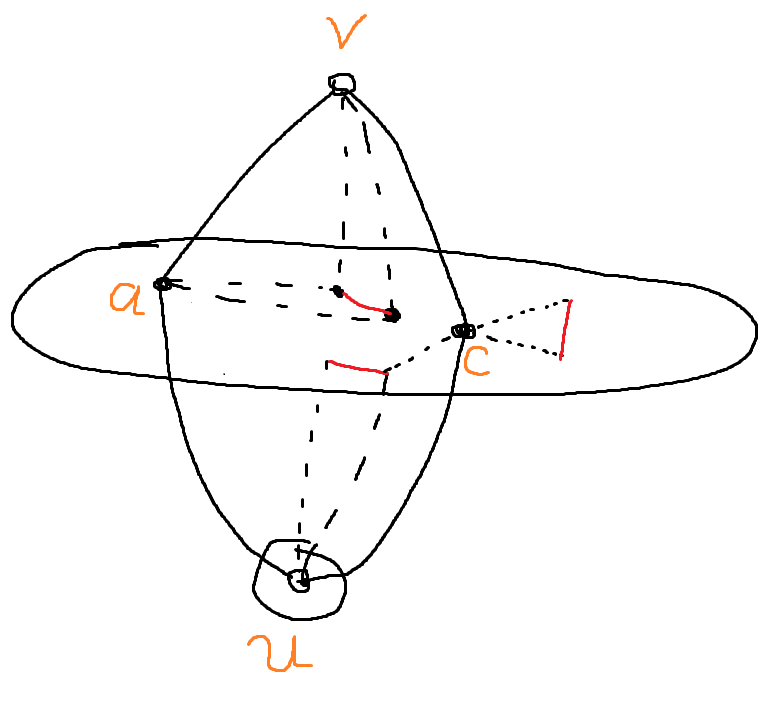
\includegraphics[width = 11cm, height = 8cm]{im1.png}
	\item Красные рёбра - добавленные при вырезании квадрата.
	\item Другими словами: правильность раскраски следует из теоремы о существовании правильной списочной раскраски (у каждой вершины списки размера 2), а динамичность - по индукции и добавленным рёбрам.
	\item Осталось разобрать второй случай.
	\item Случай 2: $(N_G(a) \cap N_G(c))\setminus v = \emptyset$
	\item Тут кажется следует действовать так:
	\item Раз у нас нет этого квадрата, сделаем его сами. Для этого достаточно придумать как встроить вершину u, \sout{не привлекая внимание санитаров} не увеличив максимальную степень графа $\Delta(G)$
	\item to be continued, hopefully.
	\end{itemize}
	\hfill $\square$\\
\end{document}
	
	